\documentclass[a4paper,12pt]{article}

\usepackage[utf8x]{inputenc}
\usepackage[english, russian]{babel}

\usepackage{tabularx}
\usepackage{multirow}
\usepackage{graphicx}

\usepackage{diagbox}

\usepackage{makecell}
\usepackage{indentfirst}


\usepackage{textcomp}
%\usepackage{literat}

\usepackage{fullpage}

\usepackage{amsmath}
\usepackage{amsfonts}
\usepackage{amssymb}

\exhyphenpenalty=10000
\doublehyphendemerits=10000
\finalhyphendemerits=5000

\begin{document}

\begin{titlepage}
\newpage

\

\begin{center}
	\large		
   	Министерство образования и науки Российской Федерации\\[0.5cm]
    	
	ФГБОУ ВО Рыбинский государственный авиационный технический университет имени П.А. Соловьева\\[1.0cm]

	Факультет радиоэлектроники и информатики\\[0.25cm]
		
	Кафедра математического и программного обеспечения\\ электронных вычислительных средств\\[1.5cm]

	\Large
	\textbf{\textsc{ОТЧЕТ ПО ЛАБОРАТОРНОЙ РАБОТЕ}}\\[0.25cm]
	по  дисциплине\\
	\textbf{Математические методы анализа данных}\\[0.5cm]
	
	по теме\\
	Предварительная обработка значений временных рядов\\ Определение наличия тренда

\end{center}

\vfill	
\begin{tabularx}{0.95\textwidth}{lXr}
Студент группы ИПБ-13 			& &	Иванов Р.А. \\
Преподаватель, доцент	& & Воробьев К. А.\\
\end{tabularx}

\vspace{1.5cm}
\center Рыбинск 2017
\end{titlepage}	


\newpage
\setcounter{page}{2}

\tableofcontents

\newpage\section{Аномальные значения. Критерий Ирвина}
Аномальные значения временного ряда не отвечают потенциалу исследуемой системы, и их использование для построения трендовой модели может сильно исказить получаемые результаты. Причинами появления аномальных уровней могут быть технические ошибки при сборе, обработке и передаче информации. Такие ошибки называются ошибками первого рода, их можно выявить и устранить или принять меры к их недопущению. Кроме того, аномальные уровни могут возникать из-за воздействия факторов, имеющих объективный характер, но действующих эпизодически. Такие ошибки называются ошибками второго рода, их невозможно устранить, но можно исключить из рассмотрения, заменив аномальное значение на среднеарифметическое двух соседних уровней.

\vspace{0.5cm}
Для выявления аномальных значений ряда используется критерий Ирвина, согласно которому аномальной считается точка $Y_t$, отстоящая от предыдущей точки $Y_{t-1}$ на величину, большую среднеквадратичного отклонения($\sigma$)

$$\lambda_i = \frac{|Y_i - Y_{i-1}|}{\sigma}$$

Точка считается аномальной, если $\lambda_i$ больше табличного $\lambda_t$.

\vspace{0.5cm}
В качестве исходных данных использована  история котировки USDEUR за период с мая 2014 по май 2016 включительно с периодичностью(временной разницей между соседними измерениями) в 1 неделю(всего 100 значений котировки).
В рассматриваемом ряде максимальное значение $\lambda_i$ составило $0,598302944222597$, т.е. аномальные точки отсутствуют.

\newpage\section{Методы сглаживания}
Очень часто уровни ряда динамики колеблются, так что тенденция развития процесса скрыта случайными отклонениями. 

\vspace{0.5cm}
Сглаживание временного ряда позволяет отфильтровать мелкие случайные колебания и выявить основную тенденцию изменения исследуемой величины. При механическом сглаживании выравнивание отдельных уровней производится с использованием значений соседних уровней. Для сглаживания используются следующие методы.

\subsection{Простая (среднеарифметическая) скользящая средняя}
$$\tilde{Y}_i = \frac{\sum\limits_{j=i-p}^{i+p}Y_j}{2p + 1}$$

\subsection{Взвешенная (средневзвешенная) скользящая средняя}
$$\tilde{Y}_i = \frac{\sum\limits_{j=i-p}^{i+p}\rho_jY_j}{\sum\limits_{j=i-p}^{i+p}\rho_j}$$

В этом методе каждая из точек входит в общую сумму с весовым коэффициентом $\rho_i$. Для сглаживания по $5$ точкам используют весовые коэффициенты $(-3, 12, 17, 12, -3)$. Для сглаживания по $7$ точкам используются коэффициенты $(-2, 3, 6, 7, 6, 3, -2)$.

\subsection{Среднехронологическая}
$$\tilde{Y}_i = \frac{\frac{Y_{i-p}}{2} + \sum\limits_{j=i-p+1}^{i+p-1}Y_j+\frac{Y_{i+p}}{2}}{2p}$$

\subsection{Экспоненциальное сглаживание}
В этом методе для сглаживания текущей точки используются все предшествующие точки, причем значения весовых коэффициентов убывают по экспоненте по мере удаления от текущей точки. Используя рекуррентные соотношения, получим выражение для текущей сглаженной точки как функцию от текущей несглаженной точки и предыдущей сглаженной:
$$\tilde{Y}_i = \alpha Y_i - (1 - \alpha)\tilde{Y}_{i-1}$$ 
где $\alpha$ – параметр сглаживания. В качестве $\tilde{Y}_1$ можно взять $Y_1$.


\newpage
На графиках представлена выборка в исходном виде и после применения описанных выше методов сглаживания(рис. \ref{fig:im_1} - \ref{fig:im_2}).

\begin{center}
	\begin{figure}[h]
		\centering
   		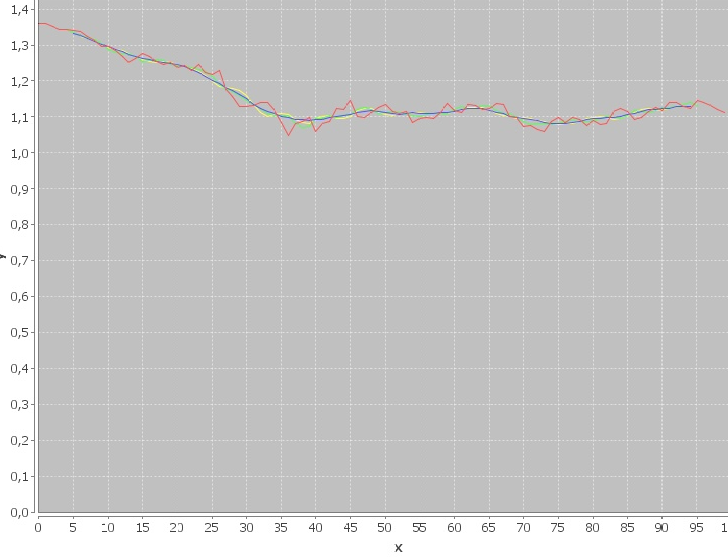
\includegraphics[scale=0.9]{figure_1.png}
   		\caption{исходная выборка(красная линия), среднеарифметическая по 5 точкам(синяя), средневзвешанная по 5 точкам(зеленая), средневзвешанная по 7 точкам (желтая)}
   		\label{fig:im_1}
    \end{figure}
\end{center}
\newpage
\begin{center}
	\begin{figure}[h]
		\centering
   		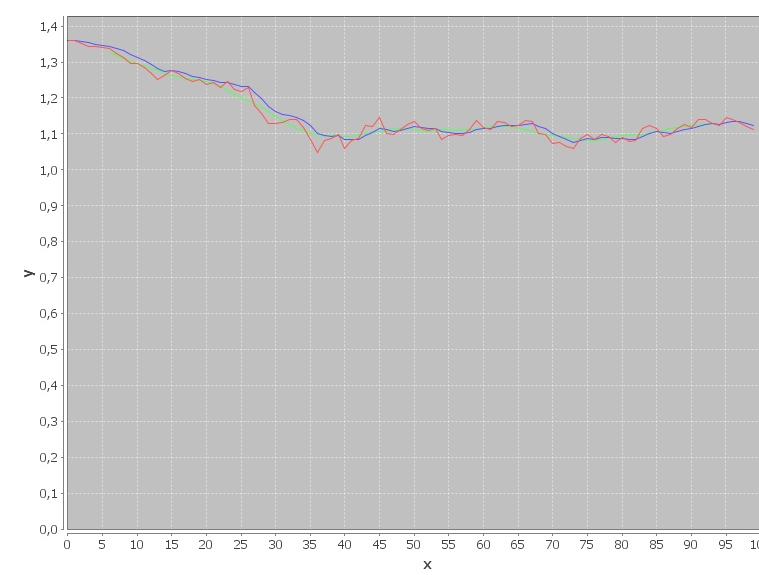
\includegraphics[scale=0.9]{figure_2.png}
   		\caption{исходная выборка(красная линия), среднехронологическая по 12 точкам(синяя), экспоненциальное сглаживание(зелёная)}
   		\label{fig:im_2}
    \end{figure}
\end{center}

\newpage
\section{Методы определения наличия тренда}
Под словом тренд понимается основная тенденция изменения временного ряда.\\Тренды могут быть описаны различными уравнениями — линейными, логарифмическими, степенными и т.д. Фактический тип тренда устанавливают на основе подбора его функциональной модели статистическими методами либо сглаживанием исходного временного ряда.

\vfill
\subsection{Метод проверки разностей средних уровней}
Разделим исходный ряд из $n$ точек на два с примерно одинаковым числом точек $n_1$ и $n_2, (n = n_1 + n_2)$ и для каждой из частей вычислим средние значения и дисперсию

\vspace{0.5cm}
Проверим гипотезу об однородности дисперсий частей ряда с помощью критерия Фишера:
$$F = \left\{\begin{array}{ll}
	\frac{\sigma_1^2}{\sigma_2^2}, & \sigma_1^2 > \sigma_2^2\\
	\frac{\sigma_2^2}{\sigma_1^2}, & \sigma_2^2 > \sigma_1^2\\	
\end{array}\right.$$
 
\vspace{0.5cm}
Если полученное значение $F$ меньше табличного $F_t$, то гипотеза об однородности дисперсий принимается и переходят к следующему этапу расчета. Если $F$ больше или равно табличному значению $F_t$, то гипотеза об однородности дисперсий отклоняется и метод не дает ответа на вопрос о наличии или отсутствии тренда.

Окончательная проверка гипотезы об отсутствии тренда производится с использованием $t$-критерия Стьюдента, вычисляемого по формуле
$$t = \frac{|\bar{Y}_1 - \bar{Y}_2|}{\sigma \sqrt{\frac{1}{n_1} + \frac{1}{n_2}}}$$
где $\sigma = \sqrt{\frac{(n_1 - 1)^2\sigma_1^2 + (n_2 - 1)^2\sigma_2^2}{n_1 + n_2 - 2}}$ - среднеквадратическое отклонение разности средних

\vspace{0.5cm}
Если расчетное значение $t$ меньше табличного значения $t_t$, то гипотеза принимается, т.е. тренда нет, в противном случае тренд есть. 

\vspace{0.5cm}
В данном случае значение коэффициента $F$ составило 19,041836213951203, что значительно больше табличного( 1.3917), т.е. метод не позволяет установить наличие или отсутствие тренда.
\vfill

\newpage
\subsection{Метод Фостера-Стьюарта}
Этот метод дает более надежные результаты по сравнению с предыдущим. Кроме самого тренда он позволяет установить наличие тренда дисперсии. При отсутствии тренда дисперсии разброс уровней ряда постоянен, при наличии тренда дисперсии дисперсия увеличивается или уменьшается.

\vspace{0.5cm}
Выполним сравнение каждого уровня ряда с предыдущим и определим две последовательности
$$\begin{array}{c}
	k_t = \left\{\begin{array}{ll}
		1, & Y_t > \max\limits_{i=1}^{t-1}Y_i\\
		0, & else
	\end{array}\right.\\
	l_t = \left\{\begin{array}{ll}
		1, & Y_t < \min\limits_{i=1}^{t-1}Y_i\\
		0, & else
	\end{array}\right.
\end{array}$$

\vspace{0.5cm}
Вычислим величины $s$ и $d$, характеризующие изменение временного ряда и дисперсии
$$s = \sum\limits_{i=1}^n (k_i + l_i)$$
$$d = \sum\limits_{i=1}^n (k_i - l_i)$$
 
Величина $s$ характеризует изменение временного ряда, она может принимать значение от $0$ (когда все уровни ряда равны) до $n - 1$ (ряд монотонный). Величина $d$ характеризует изменение дисперсии временного ряда и изменяется от $-(n - 1)$ (когда ряд монотонно убывает) до $(n - 1)$ (когда ряд монотонно возрастает). Эти величины являются случайными с математическим ожиданием $\mu$ для значения $s$ и $0$ для значения $d$.
Проверим гипотезы о случайности отклонения величины $s$ от ее математического ожидания $\mu$ и о случайности отклонения величины $d$ от нуля с помощью критерия Стьюдента для средней и для дисперсии
$$t_s = \frac{|s - \mu|}{\sigma_1}, \quad \sigma_1 = \sqrt{2\ln n - 3.4253}$$
$$t_d = \frac{|d - 0|}{\sigma_2}, \quad \sigma_2 = \sqrt{2\ln n - 0.8456}$$
 
 
где $\mu$ – математическое ожидание величины $s$ для случайного временного ряда $\sigma_1$ – среднеквадратичное отклонение $s$ для случайного временного ряда, $\sigma_2$ – среднеквадратичное отклонение $d$ для случайного временного ряда.

\vspace{0.5cm}
Полученные значения $t_s$, $t_d$ необходимо сравнить с табличными значениями критерия Стьюдента $t_t$. Если $t_t$ больше расчетного значения, то соответствующий тренд отсутствует.

\vspace{0.5cm}
Выполнив рассчёты было получено, что $s = 23$, $d = -21$, $t_s = 6,569070002559809$, $t_d = 7,260943575402728$. Последние 2 параметра значительно превышают значение $t_t$(1.984), что явно говорит о наличии тренда.

\newpage\section{Выводы}

Использование метода проверки разностей средних уровней не дало какой-либо информации о наличии или отсутствии тренда. Однако метод Фостера-Стьюарта, который не даром считается более надёжным, указал на наличие тренда как среднеарифметического, так и дисперсии. Положительное значения коэффициентов $s$ и отрицательное $d$ говорят о наличи нисходящего тренда, о котором можно было предположить по виду графика. 


\end{document}